\section{بخش اول: آمار تصاویر (\lr{Image Statistics})}

\begin{stepbox}
\field{مقدمه و آماده‌سازی داده‌ها}{
در این بخش از مجموعه داده‌ی (\lr{CIFAR-10}) شامل تصاویر رنگی با ابعاد $32 \times 32 \times 3$ استفاده شده است. هدف، پیاده‌سازی دستی آماره‌های بنیادی شامل میانگین تصویر (\lr{Mean Image})، میانگین شدت روشنایی (\lr{Mean Intensity})، واریانس (\lr{Variance})، انحراف معیار (\lr{Standard Deviation}) و هیستوگرام (\lr{Histogram}) بدون استفاده از توابع سطح بالای آماری مانند \texttt{numpy.mean} یا \texttt{numpy.var} است.
}
\end{stepbox}

\begin{codebox}[محاسبه‌ی دستی آماره‌های بنیادی داده‌ها]
\begin{lstlisting}[language=Python]
import numpy as np
import matplotlib.pyplot as plt
from tensorflow.keras.datasets import cifar10

(x_train, y_train), _ = cifar10.load_data()
images = x_train.astype(np.float64)

# 1. Mean Image (تصویر میانگین در ابعاد 32x32x3)
mean_img = np.sum(images, axis=0) / images.shape[0]

# 2. Mean Intensity (میانگین شدت روشنایی کل پیکسل‌ها)
pixels_per_channel = images.shape[0] * images.shape[1] * images.shape[2]
sum_per_channel = np.sum(images, axis=(0, 1, 2))
mean_intensity = sum_per_channel / pixels_per_channel

# 3. Variance (واریانس شدت روشنایی به تفکیک کانال)
variance = np.sum((images - mean_intensity)**2, axis=(0, 1, 2)) / pixels_per_channel

# 4. Standard Deviation (انحراف معیار)
std_dev = np.sqrt(variance)
\end{lstlisting}
\end{codebox}

\begin{notebox}[منطق ریاضی مرکزگرایی (\lr{Mean Subtraction})]
از نظر ریاضی، تفریق تصویر میانگین از تمامی نمونه‌ها ($X_i - \bar{X}$) سبب خنثی‌سازی مولفه‌ی ایستای پس‌زمینه (\lr{DC Bias}) می‌گردد. این امر موجب تمرکز الگوریتم‌های یادگیری عمیق بر روی تغییرات ساختاری و بافت‌های محلی شده و از انحراف گرادیان‌ها در طول فرآیند آموزش جلوگیری می‌کند.
\end{notebox}

\subsection{تحلیل هیستوگرام و توزیع شدت روشنایی}

\begin{figure}[htbp]
    \centering
    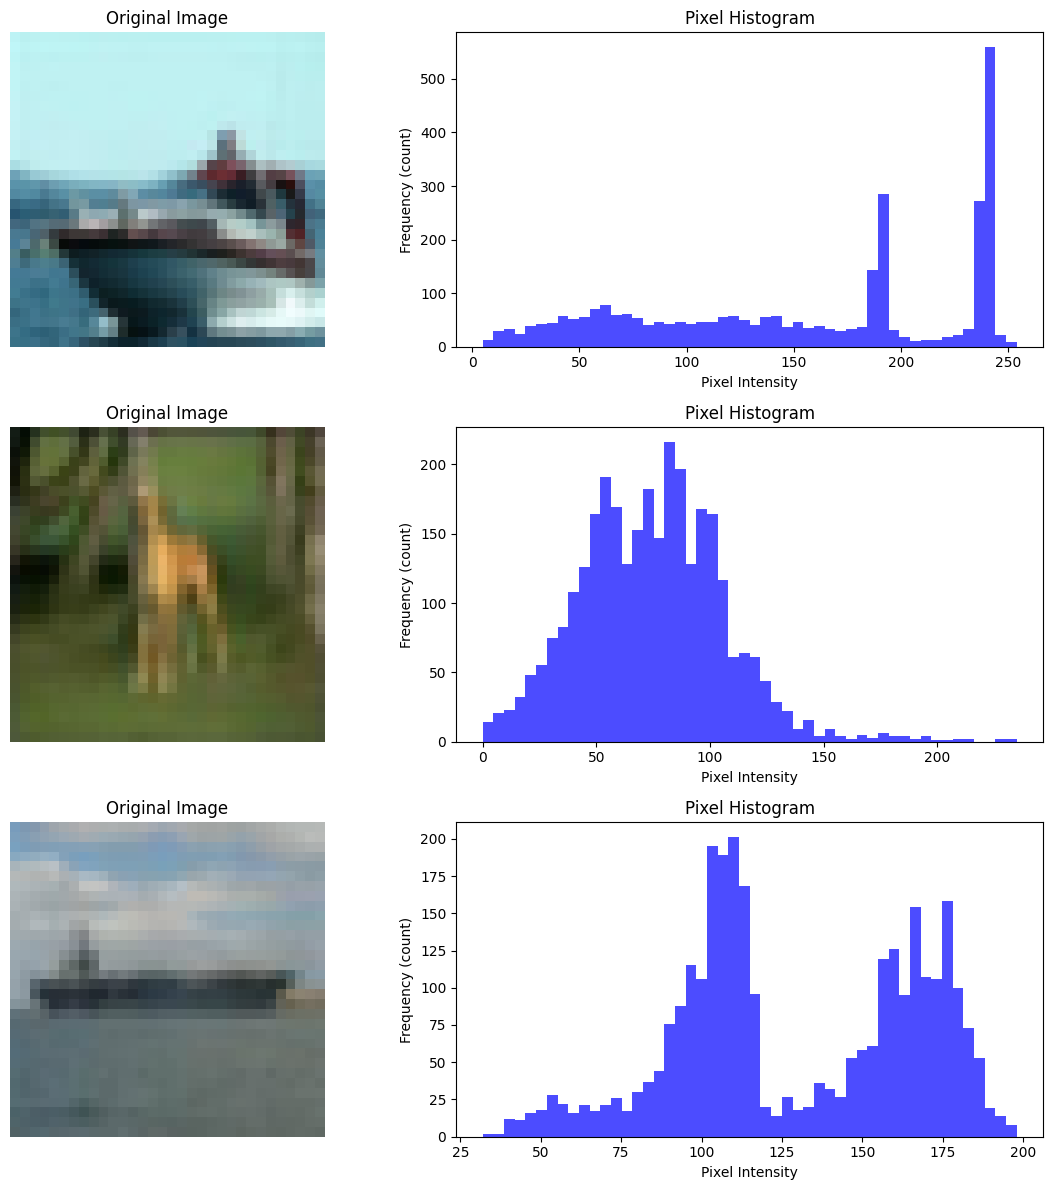
\includegraphics[width=0.82\textwidth]{images/img_hist_original.png}
    \caption{نمایش تصویر نمونه و هیستوگرام شدت روشنایی پیکسل‌های آن}
    \label{fig:hist_original}
\end{figure}

\begin{stepbox}
\field{پاسخ به سوالات تحلیلی}{
\textbf{۱. کدام تصاویر روشن‌تر هستند؟} \\
تصاویری که مرکز ثقل توزیع روشنایی آن‌ها (\lr{Mean Intensity}) به سمت مقادیر انتهایی طیف (نزدیک به ۲۵۵) تمایل دارد، روشن‌تر هستند. در هیستوگرام، تجمع پیکسل‌ها در سمت راست محور افقی نشان‌دهنده‌ی نوردهی بالا (\lr{Overexposed}) است.

\textbf{۲. کدام تصاویر کنتراست بالاتری دارند؟} \\
کنتراست مستقیماً با پراکندگی پیکسل‌ها حول میانگین یا همان \textbf{واریانس (\lr{Variance})} در ارتباط است. تصاویری که دارای واریانس بالاتری هستند، دامنه دینامیکی گسترده‌تری داشته و در هیستوگرام آن‌ها پیکسل‌ها روی کل طیف $[0, 255]$ پخش شده‌اند (گاهی به صورت توزیع دوگانه یا \lr{Bimodal Distribution}). تصاویری با واریانس پایین، هیستوگرام فشرده و تمرکز بالا حول یک نقطه دارند که نشان‌دهنده کدر بودن تصویر (\lr{Low Contrast}) است.

\textbf{۳. هیستوگرام چه اطلاعاتی را آشکار می‌سازد؟} \\
هیستوگرام در حقیقت تابع چگالی احتمال تجربی (\lr{Empirical PDF}) شدت روشنایی تصویر است. محور افقی مقدار شدت روشنایی و محور عمودی فراوانی پیکسل‌ها را نشان می‌دهد. این نمودار وضعیت نوردهی، کنتراست، دامنه دینامیکی و حد تفکیک‌پذیری عارضه از پس‌زمینه را بدون وابستگی به موقعیت مکانی پیکسل‌ها مشخص می‌کند.
}
\end{stepbox}